% !Mode:: "TeX:UTF-8"
% !TEX program  = xelatex
\documentclass[a4paper]{article}
\usepackage{amsmath}
\usepackage{amssymb}
\usepackage{extarrows}
\usepackage{ctex}
%\usepackage{braket}
%\usepackage[european]{circuitikz}
\usepackage{multirow}
\usepackage{float}
\usepackage{graphicx}
\usepackage{wrapfig}
\usepackage{geometry}
\geometry{left=2.5cm,right=2.5cm,bottom=2.5cm,top=2.5cm}
\title{近代物理实验报告4.1:西蒙气体温度计与蒸汽压温度计}
\author{xy\quad 学号\quad 匡亚明学院}
\date{2019年2月29日}
\begin{document}
\maketitle
\bibliographystyle{unsrt}
%--------main-body------------

\section{引言}
西蒙气体温度计是一种测温范围广、结构简单、使用方便的定容气体温度计,常用于一般低温工程技术。它和用于热力学温度标准的精密气体温度计相比,主要是测量精度存在差距而在测量原理上并无多大差别。蒸气压温度计则广泛应用于低温实验室的温度测量及控制,它具有反应快、准确性好、简单方便的优点。在低温实验室用得最普遍的是氦、氧和氮的蒸气压温度计。本实验将西蒙气体温度计和氮蒸气压温度计的感温泡热学上连结在一起,共同浸入盛有液氮的杜瓦瓶中,进行低温实验的温度测量。若同时置放真实样品,在改变温度并满足热平衡的条件下,即可获得被测样品的物理特性的温度响应,例如置入高临界温度超导材料,可以获得该材料的临界电流-温度特性。

\section{实验目的}
通过实验了解气体温度计和蒸气压温度计的测温原理,学习利用这两种温度计测量低温温度的技术及误差分析,掌握低温物理实验中常用的减压降温及恒压控温的技术。

\section{实验仪器}
杜瓦瓶、抽气系统。

\section{实验原理}
\subsection{西蒙气体温度计的结构和原理}
如图(\ref{fig1})所示,西蒙气体温度计由三部分组成:
\begin{enumerate}
\item 感温泡。用紫铜加工而成,因紫铜导热性良好,可以改善温泡和待测温物体的热接触。
\item 压力指示器。采用弹簧管精密真空表。它有一弹性弯管通过杠杆链接到指针上。当管内气体压力变化时,弹簧管发生形变,带动指针指示相应的真空度,一般情况下弹簧管的体积可认为不变,因而可供制作简单的定容气体温度计。
\item 连接感温泡和压力指示器的毛细管。毛细管的作用是充当压力传输管,可选内径为0.2$\sim$0.5mm的不锈钢管。
\end{enumerate}
将毛细管分别与感温泡及真空表焊接后抽至$10^{-1}$帕量级的真空,充入氦气并置换几次,最后封入少量氦气,理想气体状态方程为
\begin{equation}
pV_m = RT\label{eq1}
\end{equation}
式中p为气体压力,$V_m$为气体摩尔体积,T为绝对温度,R为普适气体常数。在本实验中,以V代表感温泡的体积,V$^{'}$代表真空表内弹簧管的体积,以及附加的密封铅管管道的体积(总称“死体积”)。$p_0$代表室温$T_0$时气体温度计内气体压力。忽略毛细管的体积,则当感温泡浸入液氮中,温泡内气体温度下降至T,压力亦相应变为p,由(\ref{eq1})式应有
\begin{equation}
\frac{pV^{'}}{T_0} + \frac{pV}{T} = \frac{p_0V^{'}}{T_0} + \frac{p_0V}{T_0} = nR = \text{常数}\label{eq2}
\end{equation}
式中n为温度计内的气体的摩尔数。由(\ref{eq2})式可得
\begin{equation}
T = \frac{\alpha T_0p}{(1+\alpha)p_0 - p}\label{eq3}
\end{equation}
其中$\alpha$=V/V$^{'}$。如果V$^{'}$和V两者之一或两者都不知道,可由(\ref{eq3})式写成另外一种形式
\begin{equation}
\alpha = \frac{(p - p_0)T)}{p_0T - pT_0}\label{eq4}
\end{equation}
而求得。例如由其他温度计测得室温后,在温泡未置入低温温区之前,读出真空表相应于室温$T_0$的$p_0$,再读出感温泡置于液氮沸点T(已知)时真空表读数p,立即可定出。
也可以将(\ref{eq2})式写成另外的形式:
\begin{equation}
\frac{1}{T}(VT_0) + V^{'} = \frac{1}{p}(p_0^{'}V + p_0V)\label{eq5}
\end{equation}
式中$\frac{1}{T}$与$\frac{1}{p}$的关系为一直线方程。若令
\begin{equation}
\beta = \frac{p_0(V+V^{'})}{VT_0}\text{, }\theta = \frac{V^{'}}{VT_0}\label{eq6}
\end{equation}
则有
\begin{equation}
\frac{1}{T} = \beta\frac{1}{p} - \theta\label{eq7}
\end{equation}
只要求出和,利用作图法可以方便的建立p-T关系。

以上讨论的是理想气体的情形。实际为照顾真空表的读数范围,实验中所充的氦气并没有稀薄到完全可以忽略。考虑到真空气体中第二维里系数项所产生的影响,气体状态方程应为
\begin{equation}
pV_m = RT + Bp\label{eq8}
\end{equation}
比较(\ref{eq1})式和(\ref{eq8})式,温度的修正项为
\begin{equation}
\Delta T = -\frac{Bp}{R}\label{eq9}
\end{equation}
第二维里系数B的值和温度有关。

造成西蒙气体温度计的误差有多方面的因素,如真空表读数误差,热分子压差效应引起的误差,温泡体积热胀冷缩变化,处于温度梯度内的毛细管体积对值的影响等。其中真空表读数不精确是主要来源,估算时可将(\ref{eq2})式两边对p求偏导数,得到由于压力读数误差$\Delta p$而引起地误差为
\begin{equation}
\Delta T = T\left(1+\frac{T}{\alpha T_0}\right)\frac{\Delta p}{p}\label{eq10}
\end{equation}
其中p的值相对于精密真空表而言为333.3帕。若预先对准精密真空表的刻线进行压力标定,可使p值缩小为133.32帕。
\subsection{蒸气压温度计}
\begin{figure}[!h]
\begin{minipage}{0.48\textwidth}
\begin{center}
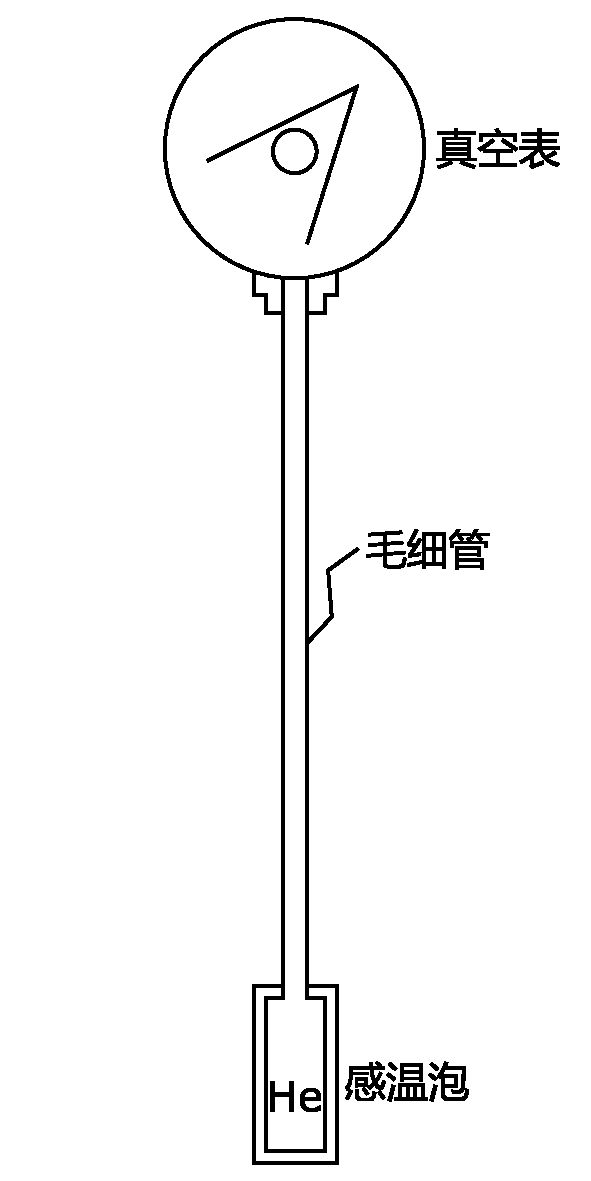
\includegraphics[width=0.6\textwidth]{fig/fig1.pdf}
\caption{西蒙气体温度计示意图}\label{fig1}
\end{center}
\end{minipage}
\begin{minipage}{0.48\textwidth}
\begin{center}
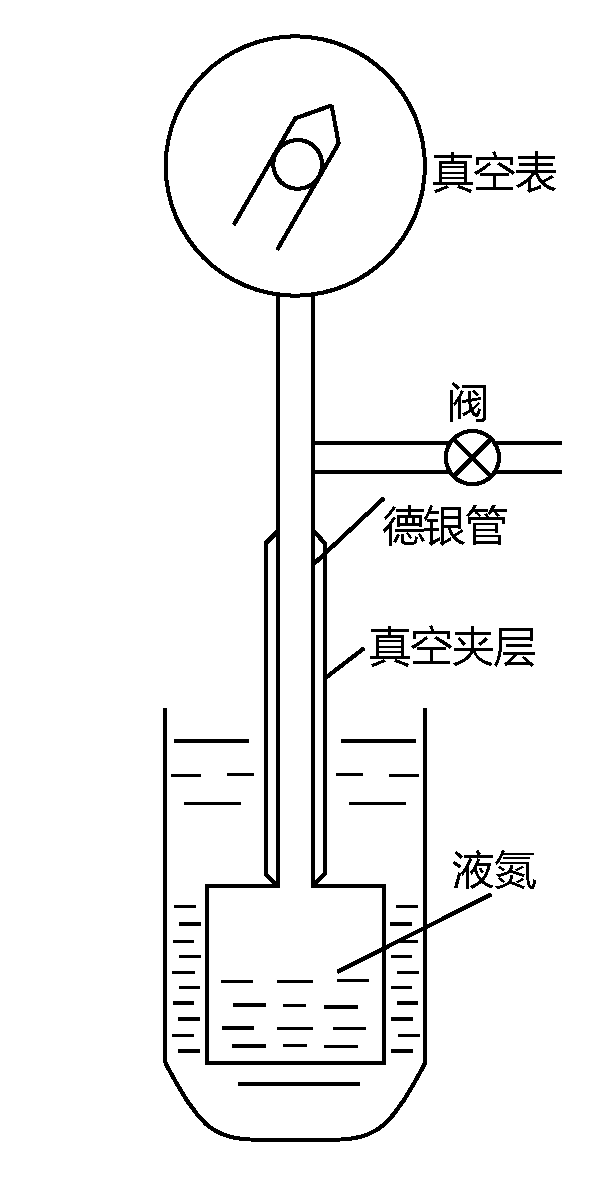
\includegraphics[width=0.6\textwidth]{fig/fig2.pdf}
\caption{氮蒸汽压温度计示意图}\label{fig2}
\end{center}
\end{minipage}
\end{figure}
如果我们借助于一台抽气机降低液体表面上的蒸气压,那么由于表面蒸气压的降低,会导致液体内部一些动能较大的分子逸出液面被抽气机抽走,从而使液体的平均动能降低,也就是说降低了液体的温度。根据热力学的相平衡理论,单元两相系在相平衡时温度和压力之间存在一一对应的关系,为获得表达液体的这种关系的蒸气压方程,可对克劳修斯-克拉贝龙(Clausius-Clapeyron)方程积分,积分后的系数要借助于气体温度计来标定。对于氮蒸气压温度计,其饱和蒸气压与温度的关系为
\begin{equation}
\text{lg}p = 7.781845 - \frac{341.619}{T} - 0.0062649T\label{eq11}
\end{equation}
一般来说重力场及环境温度变化对其引起的偏离很小。

图(\ref{fig2})为本实验所用的氮蒸气压温度计。它由一浸于液氮中待测温区的温泡和置于杜瓦瓶上方的精密真空表以及连接这两者的德银管组成。温泡内充以一定量的纯净液氮;带有真空夹层的德银管作为传递压力的管道;精密真空表用来指示感温泡内液氮蒸气的压力。对于纯净液体的缓慢降温过程,液体上部先冷,下部较热,在重力作用下产生自然对流,能使温度较快达到平衡。这时测得的温度可以认为就是浸于液氮中待测样品的温度。

\section{实验内容}
\begin{enumerate}
\item 制作氮蒸气压温度计。对氮气皮囊10充灌99.9\%以上纯度的氮气,并夹紧夹子$V_4$。调整$V_2$使得蒸气压温度计与抽气机之间处于连通状态而与其他通路处于关闭状态。启动机械真空泵,此时真空表5将指出相应的真空度。关闭阀门$V_2$,观察真空表5的指针,真空度应无明显变化。若真空表5指示的真空度明显下降,则应进行漏气检查。确定氮蒸气压温度计及其连接管道无漏气后即可松开夹子V4,此时纯氮气进入氮蒸气压温度计的各部位,准备工作完毕。
\item 记下室温、大气压力及真空表6的读数,应该注意到目前市售的真空表大多指示的是大气压力与真空表内压力之差。
\item 将贮存于液氮贮藏罐内的液氮输入实验杜瓦瓶1内。
\item 堵住输液孔15和出气孔17,调节阀门$V_1$、$V_2$、$V_3$使真空泵只对杜瓦瓶1进行抽气。随着杜瓦瓶1内蒸气压的降低,蒸气压温度计感温泡2内的氮气逐渐液化,使得皮囊10内的氮气不断进入感温泡内,直至完全液化,此时氮蒸气压温度计已可供使用。
\item 关闭抽气机,对电阻加热器接通电源。此时液氮温度逐渐回升。当真空表14指针指示杜瓦瓶内的液氮蒸气压已达大气压力时,停止加热并打开出气孔。
\item 测出氮沸点时西蒙气体温度计的读数后,再堵上出气孔17,然后抽气降温。在降温过程中利用恒压器将压力稳定在待测点后记下真空表5、6及14的读数,并换算成所测的相应温度。
\item 当液氮温度降至氮三相点温度时,通过杜瓦瓶的窥缝观察液氮表面相变情景。
\item 利用电阻8加热升温,当升温至预定测温点附近时,停止加热,让杜瓦瓶的液氮温度有一个平衡过程,记下西蒙温度计和氮蒸气压温度计数值。然后再升温,测量下一个温度点直至氮沸点。
\item 有条件时,可以从输液孔插入一只高临界温度氧化物超导材料,观察其临界电流随温度的变化。
\end{enumerate}

\section{注意事项}
\begin{enumerate}
\item 应尽量选用较纯液氮,若液氮不纯,则应注意如下两点。
\begin{enumerate}
\item 沸点偏高。此时可借助于由纯净氮气被液化的氮蒸气压温度计校正西蒙气体温度计的参数。
\item 因不纯液氮中的杂志为液氧。其沸点高达90K,在抽气降温过程中总是沸点较低的液氮蒸汽被抽走,故而纯度越来越差,降温至氮三相点时观察不到液氮结晶的物理现象,但可以观察氮、氧混合液体由透明至浑浊粘稠直至固化的物理现象,其固化点温度视液氮的杂质含量而定,通常为 59K$\sim$63K。
\end{enumerate}
\item 测量过程中室温及大气压可能会变化,应随时记录并做修正。
\item 仔细熟悉三通阀门V1及$V_2$的各种连通状况,防止误操作。
\item 在对杜瓦瓶中的液氮抽气降温时,由于气流通过三通阀门V1时的伯努利作用,可能会使乳胶指套11猛烈膨胀破裂。为此阀门$V_3$应经常处于关闭状态,只在需进一步降温时短暂开启一下,随即关闭。而在降温时,需打开$V_3$,以免乳胶指套膨胀破裂。
\end{enumerate}

\section{实验数据}

\section{误差分析}

\section{思考题}
\subsection{如何确定西蒙气体温度计感温泡体积V与“死体积”V’之比值?}
$\alpha$可由下式求得
\begin{equation*}
\alpha = \frac{(p - p_0)T)}{p_0T - pT_0}
\end{equation*}
具体来说,先用其他温度计测得室温,这样可以读出真空表相应于室温$T_0$的$p_0$,再读出感温泡置于液氮沸点T(已知)时真空表读数p,立即可定出$\alpha$。
\subsection{如果输入液氮杜瓦瓶的液氮不纯,如何正确选取氮沸点温度?}
再用纯液氮制作氮蒸气压温度计,并用此蒸气压温度计对不纯氮的结果进行校准。
\subsection{氮蒸气压温度计是如何制作的?试从氮的压力温度状态图分析其制作过程。}
先用抽气机将蒸气压温度计抽真空,然后打开夹子,此时与蒸气压温度计相连通的氮气皮囊中的纯氮气灌入蒸气压温度计各部分,之后在杜瓦中加入液氮并抽气降温,如图(数据图)所示,由于温度下降,蒸气压温度计内的氮气不断由气相进入液相,使得皮囊内的氮气不断进入蒸气压温度计的感温泡,直至完全进入,蒸气压温度计制作完成。
\subsection{本实验的恒压器是怎样工作的?}
在A、B两管之间,接有一段医用乳胶手指套,抽气降温时关闭阀门$V_3$并使三通阀门V1处于三个方向连通的状态。此时因恒压器内的乳胶指套内外存在压力差,使得乳胶指套被压缩,从而断开抽气通道。打开阀门$V_3$则恒压器内指套外压力降低,指套张开,抽气速率增大。当压力降至需要值$p_n$时关闭阀门$V_3$,则恒压器空腔内的气压维持在$p_n$处。
\subsection{本实验中观察到哪些相变现象?试描述之。}
加热到氮蒸气压等于外界大气压时,液氮沸腾,氮由液态迅速转化为气体;
抽气降温时,由于温度和压强都在下降,液氮仍继续沸腾,但随温度不断下降,观察液氮表面开始凝固,此时达到三相点。
\subsection{在抽气降温过程中,利用恒压器能使温度稳定在什么范围?是如何观测的?}
利用恒压器能使温度稳定在77K-63K之间,抽气过程中,适当松开阀门$V_3$后关闭,此后随着抽气进行乳胶指套缩小至闭合,温度将稳定在一个数值,观测数据并记录,重复上述步骤记录5-6组数据直至达到三相点。
\subsection{在升温测量过程中是如何实现稳态测量的?}
利用电阻8加热升温,当升温至预定测温点附近时,停止加热,让杜瓦瓶的液氮温度有一个平衡过程,使各个温度计达到热平衡,从而可以实现稳态测量。
\subsection{定量分析两种温度计因压力表的精度限制所致的测温误差。}
\subsubsection{对于西蒙气体温度计}
将(\ref{eq2})式两边对p求偏导数
\begin{equation*}
\Delta T = T\left(1+\frac{T}{\alpha T_0}\right)\frac{\Delta p}{p}
\end{equation*}
其中p的值相对于精密真空表而言恒定为333.3帕。若预先对准精密真空表的刻线进行压力标定,可使p值缩小为133.32帕。由此可得
\begin{equation*}
\frac{\Delta T}{T} = 1.0062\times\frac{\Delta p}{p}
\end{equation*}
可见西蒙气体温度计的相对误差不随温度变化。

\subsubsection{对于氮蒸气压温度计}
将式(\ref{eq11})两边微分得:
\begin{equation*}
\frac{\Delta T}{T} = \frac{1}{\text{ln10}}\frac{T}{341.619 - 0.0062649T^2} \xlongequal{\text{记为}}{} f(x)
\end{equation*}
可见蒸气压温度计的相对误差与温度有关,温度趋向于零时,相对误差也趋向于零,但温
度较大时相对误差较大。

由下图可知,氮蒸气压温度计适合工作在低温范围。当温度小于201.6K时,氮蒸气压温度
计的精度高于西蒙气体温度计。

\nocite{jiaocai}
\bibliography{ref}
\end{document}